\section{Design}
\label{sec:design}
Our design is built of relatively large submodules, so that not many additional elements are necessary in the top module. The structure can be seen in Fig. \ref{fig:processoroverview}. The main modules are the instruction decoder, the register file, the ALU, the memory interface and the inctruction fetch module. These modules will be described in detail in the following.

\begin{figure}[ht]
\centering
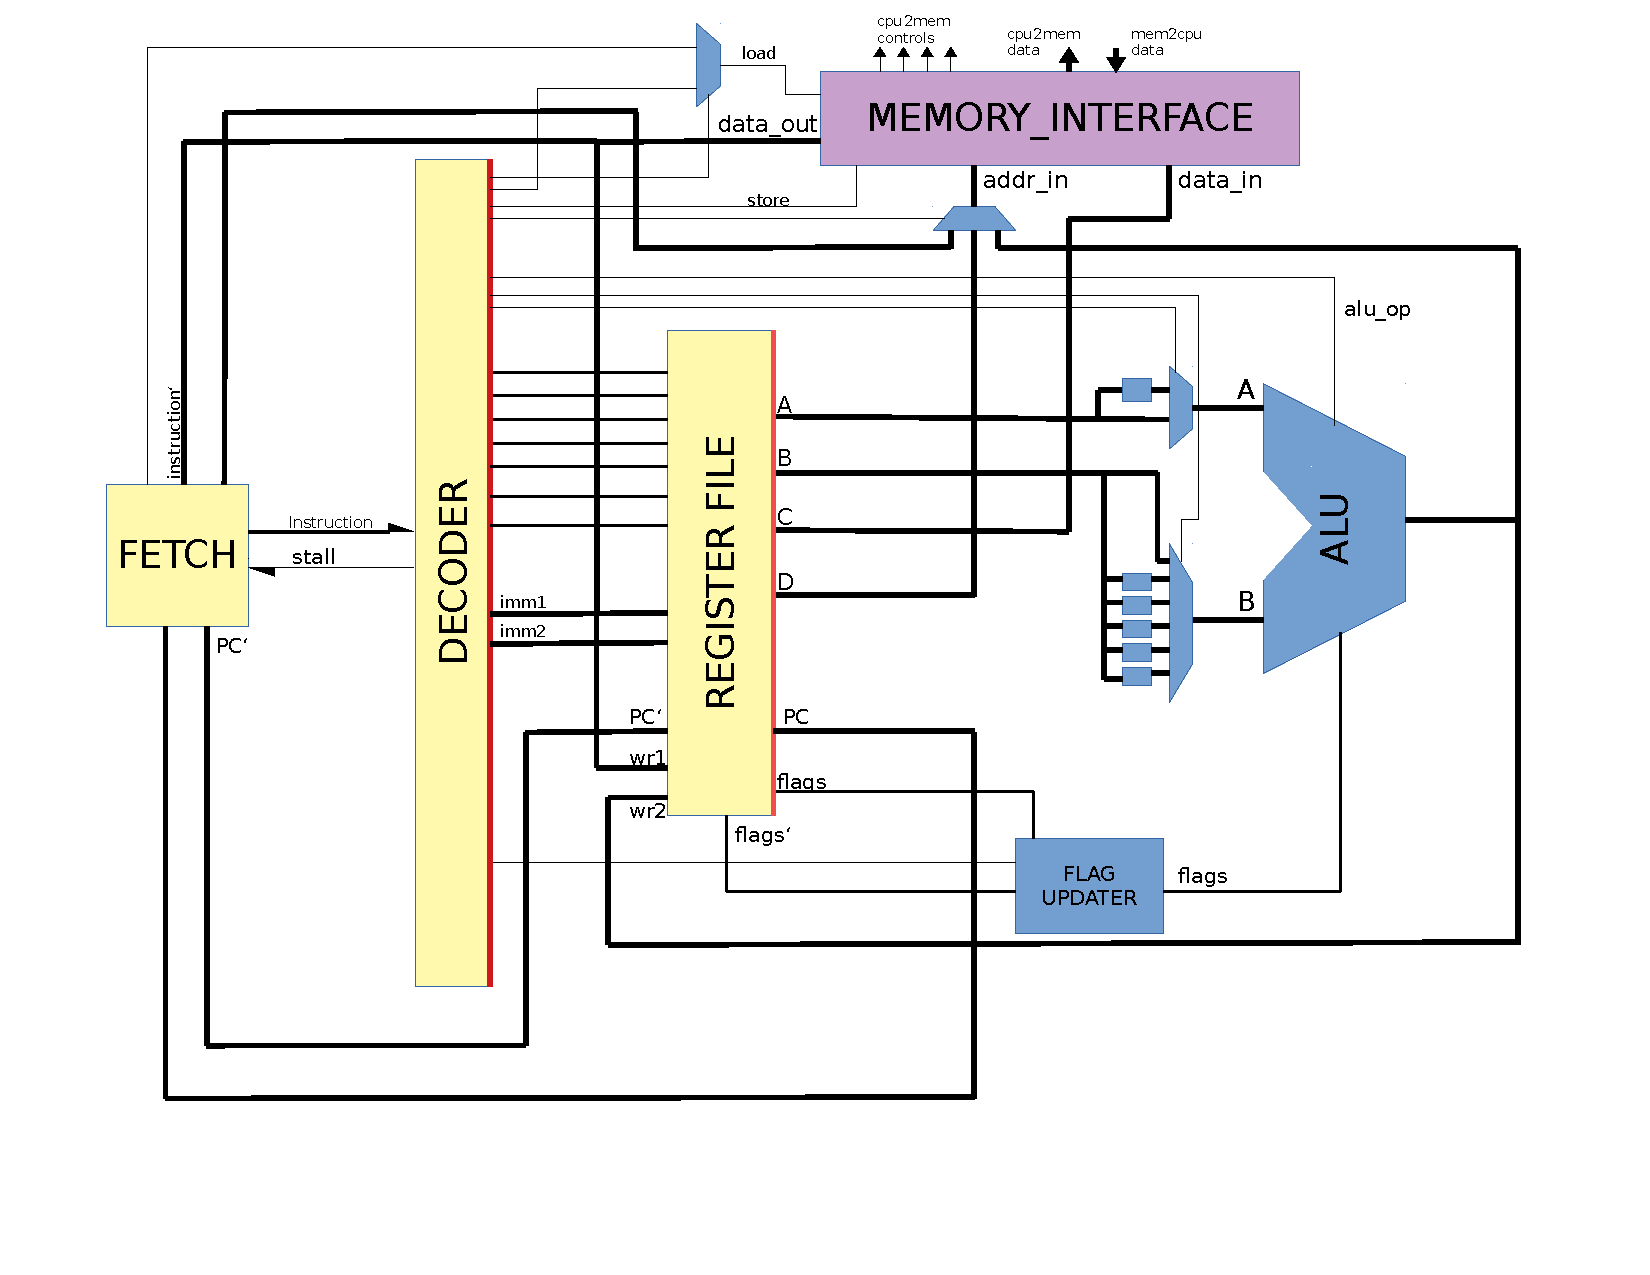
\includegraphics[scale=0.65]{images/processorOverview.pdf}
\caption{The block structure of the processor design. Register stages are marked red.}
\label{fig:processoroverview}
\end{figure}

In the block structure, the modules are connected with several connections, but only the address and load inputs for the memory are busses with more than one input. All other connections can only be driven by one module, which simplifies the overall structure. 

\subsection{Processor Control}
\label{subsec:processorcontrol}
The control of the execution and memory access is performed by a state machine in the decoder module. Initially, a dedicated controller for the memory access and pipeline stalls was planned; while integrating and testing the decoder, the function of the controller was integrated into the decoder. It yet had many control functions in order to perform multi-cycle instruction like \texttt{MULTI-PUSH/-POP}.

In general, all control signals are outputs of the decoder. These include the ALU opcode, register selects, the flag updates and memory access signals. As the memory access must be arbitrated, the decoder controls the multiplexors assigning the read request and address signals from itself and the instruction fetch module. When the current instruction accesses the memory, a stall signal to the instruction fetch can be set by the decoder. On the other hand, the instruction fetch may stall the decoder (which then stalls the rest of the processor) if the next instruction is not loaded yet. With this mechanisms, we tried to keep the control of the processor as simple as possible.

\subsection{Pipeline Stages}
\label{subsec:pipelinestages}

Our processor is comprised of two pipeline stages. One stage includes the instruction fetch and decoder, the other one does the execution and writeback tasks. These two stages have been chosen because of the structure of the benchmark applications and the 1-port memory. The applications are both relatively memory-access-loaded. The memory allows only one access per cycle; additionally, it is halfword-aligned, while the architecture uses byte-aligned addresses. The benchmarks both frequently access whole words in the memory, so that in many cycles, the memory would be the bottleneck in the execution. With only two pipeline stages, few stalls would occur. 



